When two partially miscible fluids are mixed, they tend to phase separate into distinct domains to minimize the thermodynamic penalty associated with interfacial formation. 
To inhibit this process, stabilizers such as small-molecule surfactants, particles, or biopolymers are commonly introduced. Surfactants, for example, reduce the surface tension 
between the dispersed and continuous phases, thereby lowering the interfacial energy and promoting the stability of emulsions. A familiar example is soap, which facilitates the 
emulsification of dirt into droplets suspended in water through mechanical agitation.
Without such additives, the dispersed phase tends to coalesce in order to reduce interfacial area. The effectiveness of stabilizers can be characterized through the Pieranski 
model, $G_{ads} = \sigma A_{rm} (1 - \cos{\theta_c})^2$, where $G_{ads}$ is the free energy reduction upon particle adsorption, $\sigma$ is the surface tension between the two 
fluids, and $\theta_c$ is the contact angle of the stabilizing particle. While surfactants and biopolymers reduce interfacial tension, particle stabilizers function by adsorbing 
at the interface and effectively reducing the interfacial area between fluid domains.

Compared to surfactant-stabilized emulsions, particle-stabilized emulsions (Pickering emulsions) exhibit enhanced resistance to coalescence and coarsening, prompting renewed interest 
in their use across various applications. This resurgence is further driven by increasing environmental and toxicity concerns associated with small-molecule surfactants 
\cite{kaczerewska_environmental_2020, lechuga_acute_2016}. In contrast, particle stabilizers lower toxicity and improved biocompatibility, in addition to 
sustainable sourcing from particles based on cellulose or chitin. \cite{fujisawa_nanocellulose-stabilized_2017, tang_stimuli-responsive_2016, kalliola_carboxymethyl_2018}.
The microstructure of Pickering emulsions has been extensively studied, notably by Binks and Lumsdon in the early 2000s. Their investigations revealed that the emulsion droplet radius 
follows the relationship $R_e \propto \frac{\phi_w}{\phi_p}$, where $\phi_w$ and $\phi_p$ represent the volume fractions of water and particles, respectively \cite{binks_pickering_2001}. 
They also identified key parameters influencing microstructure, such as fluid composition and particle wettability. Neutrally wetting particles tend to stabilize nearly spherical droplets, 
while non-neutrally wetting particles can induce curvature, leading to the formation of bridged droplets, capillary aggregates, and other anisotropic structures, as illustrated in 
Figure~\ref{fig:state_diagram_particle_emulsions}.

\begin{figure}
    \centering
    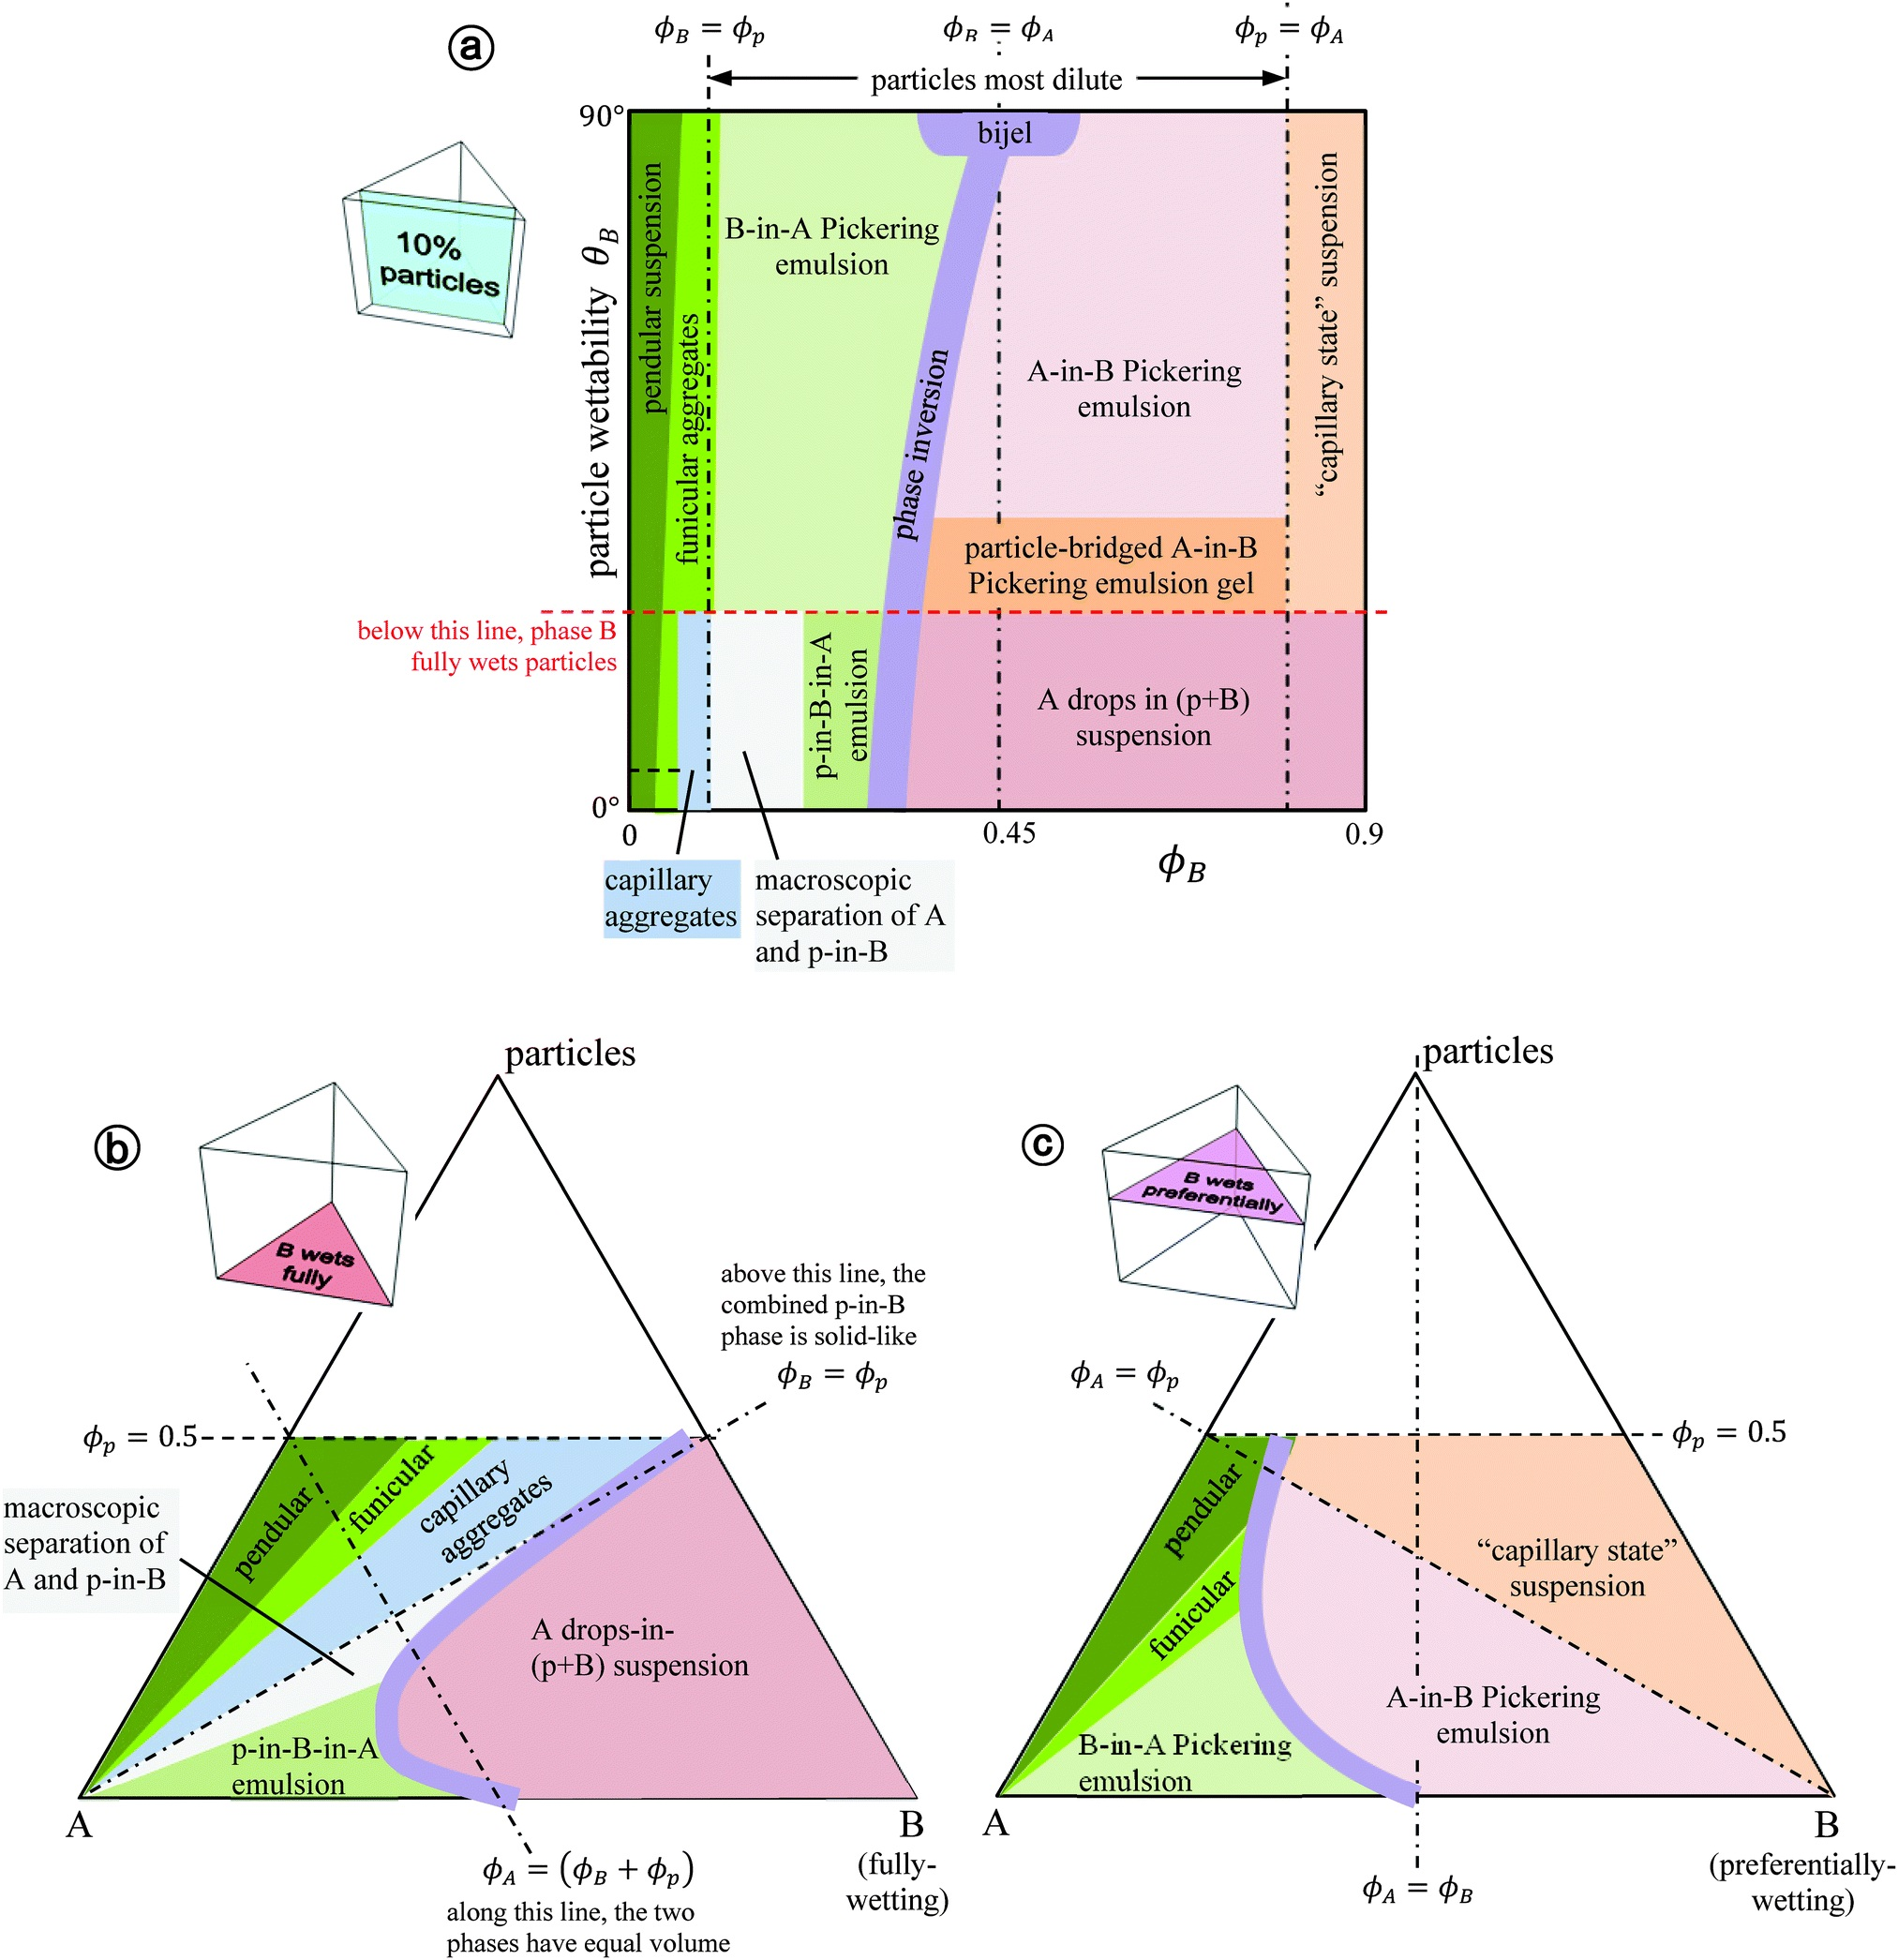
\includegraphics[scale = 0.3]{figures/literature_review/state_diagram.jpg}
    \caption{Formation criteria for a particle stabilized emulsion that can form bijel. \cite{velankar_non-equilibrium_2015}
            Used with permission of Royal Society of Chemistry, from A non-equilibrium state diagram for liquid/fluid/particle 
            mixtures, Velankar, 1, 11, 2015. Permission conveyed through Copyright Clearance Center, Inc}
    \label{fig:state_diagram_particle_emulsions}
\end{figure}

As illustrated in Figure~\ref{fig:state_diagram_particle_emulsions}, the formation of bijels typically requires a near-equal volume fraction of two immiscible fluids and neutrally wetting 
particles. 

\begin{figure}
    \centering
    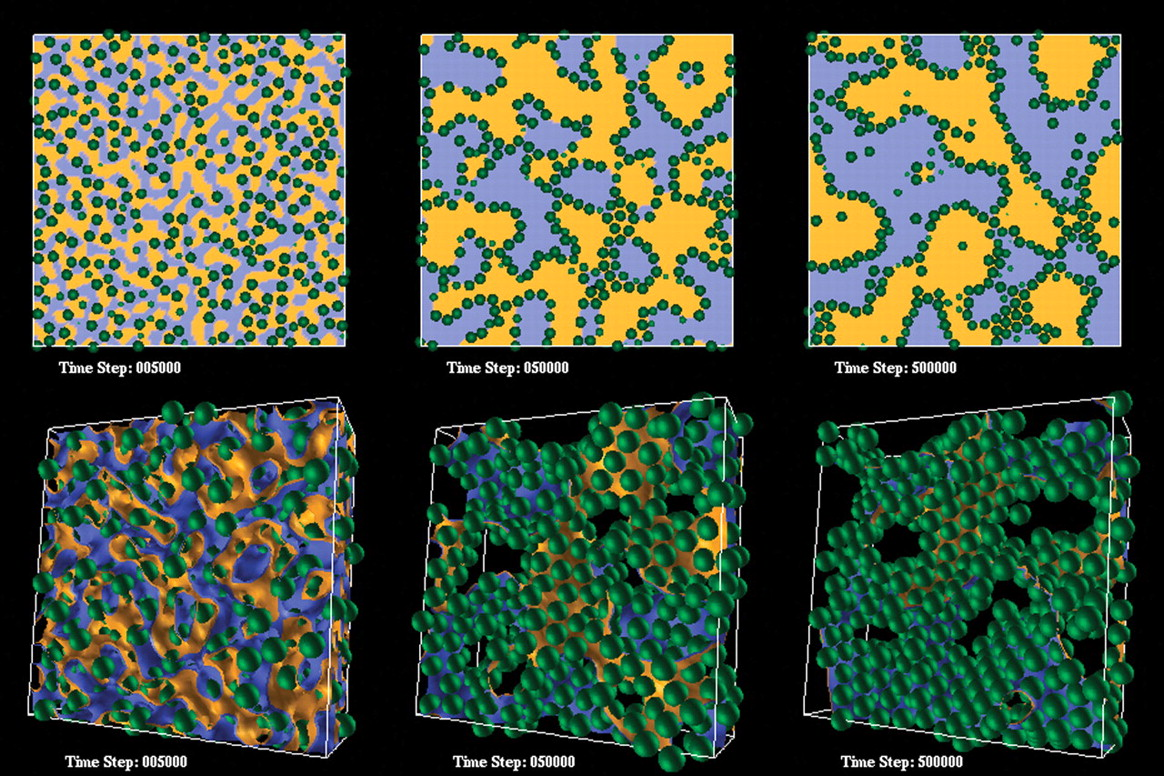
\includegraphics[scale = 0.3]{figures/introduction/bijel_coarsening.jpg}
    \caption{Initiation and arrest of spinodal decomposition as particles adsorb onto the interface, followed by jamming once the 
    interfacial area matches the cross sectional area of the adsorbed particles\cite{stratford_colloidal_2005}. 
    Reproduced from K. Stratford et al., Science 309, 2198-2201(2005) under license number 5966820525314.}
    \label{fig:bijel_coarsen}
\end{figure}

This unique microstructure was first identified in 2005 by Stratford et al., who used a multicomponent Lattice Boltzmann method coupled with suspended particles to simulate the 
dynamics of particle-stabilized emulsions under these conditions \cite{stratford_colloidal_2005}. Their simulations revealed that, following the onset of spinodal decomposition, particles 
rapidly adsorb at the evolving fluid-fluid interface. When the available interfacial area becomes comparable to the total cross-sectional area of the particles, coarsening is arrested, 
resulting in a jammed, tortuous, co-continuous morphology characteristic of bijels (see Figure~\ref{fig:bijel_coarsen}).
This computational discovery was experimentally realized in 2007 by Herzig et al., who used a 2,6-lutidine/water system stabilized with surface-modified silica particles \cite{herzig_bicontinuous_2007}. 
This binary fluid system exhibits a lower critical solution temperature (LCST) of 34.1\textdegree C and a critical composition at approximately 28\% lutidine by weight. By preparing the mixture at this 
critical composition and heating it past the LCST, phase separation was thermally induced, a process known as Thermally Induced Phase Separation (TIPS). The system underwent coarsening until gelation 
occurred, forming a bijel. Since then, a variety of small molecule, oligomeric, and polymeric systems have been developed using similar thermally induced methods 
\cite{tavacoli_novel_2011, lee_bicontinuous_2010, bai_dynamics_2015, ching_rapid_2021}. 

\begin{figure}
    \centering
    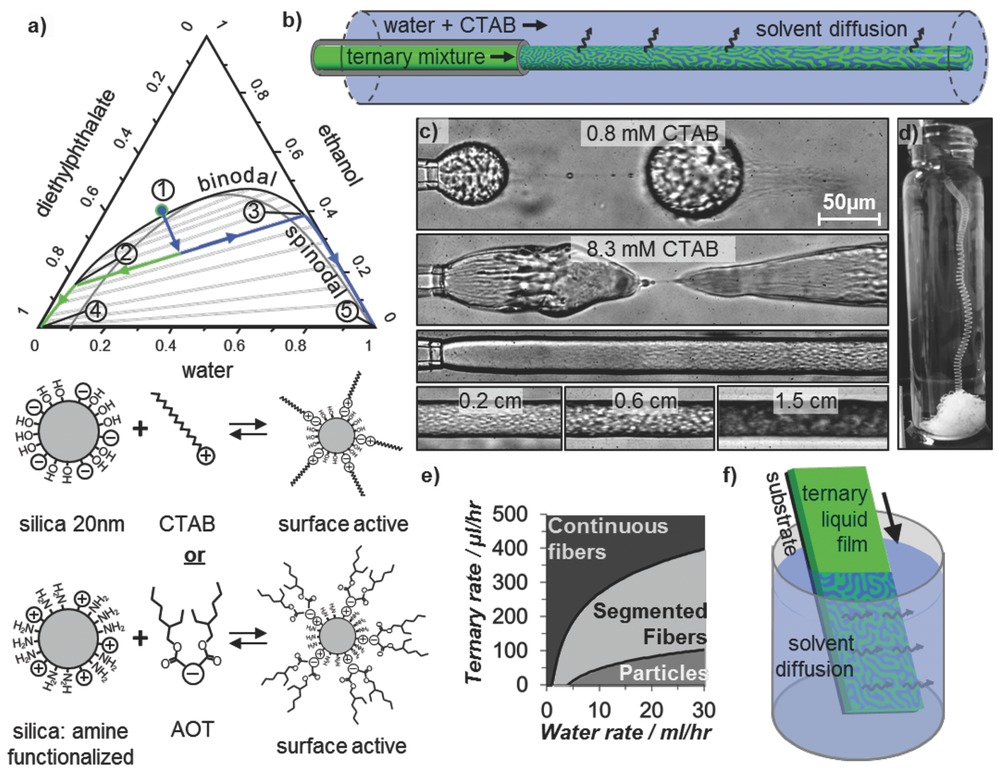
\includegraphics[scale = 5]{figures/introduction/STrIPS.jpg}
    \caption{STrIPS in action. Extrusion of the bijel casting mixture into a non-solvent bath, followed by removal of solvent from 
             the casting mixture through diffusion. \cite{haase_continuous_2015}. Reproduced with permission from Wiley-VCH Verlag GmbH 
             \& Co. KGaA from \textit{Continuous Fabrication of Hierarchical and Asymmetric Bijel Microparticles, Fibers, and Membranes by 
             Solvent Transfer-Induced Phase Separation (STRIPS)}, Haase, M. F., Stebe, K. J., 
             \& Lee, D., \textit{Advanced Materials}, 27(44), 7065-7071, 2015}
    \label{fig:strips}
\end{figure}

TIPS has been widely used in laboratory-scale studies to produce bijels in batch processes. However, industrial applications require continuous, scalable fabrication techniques capable of generating 
tailored microstructures. STrIPS has emerged as a promising solution for this need. As illustrated in Figure~\ref{fig:strips}, STrIPS involves a ternary fluid system composed of two immiscible fluids 
and a solvent. In the initial stage (Figure~\ref{fig:strips}a), a casting mixture is prepared. Phase separation is then triggered by flowing a co-solvent past the mixture to extract the solvent 
(Figure~\ref{fig:strips}b). This solvent transfer must occur within the spinodal region of the ternary phase diagram to ensure spinodal decomposition. By adjusting flow rates of both the casting 
mixture and the solvent removal stream, the resulting bijel morphology can be finely controlled. STrIPS has been successfully employed in applications ranging from battery electrode templating to drug 
delivery systems, liquid-in-liquid printing, and the creation of intrinsically polymerizable bijels for freestanding structures 
\cite{garcia_scalable_2019, thorson_bijel-templated_2019, amirfattahi_fabrication_2024, ching_rapid_2021}. The method is flexible with respect to fluid choice, with 
the only requirement being a well-characterized phase diagram that keeps the system within the spinodal regime throughout the solvent exchange process.

Vapor-induced phase separation (VIPS) offers another solvent-removal-based technique for bijel synthesis \cite{wang_scalable_2020}. In this approach, a quaternary mixture containing particles, a solvent, 
and two partially miscible liquids is prepared. Careful selection of component identities and ratios ensures that evaporation of the solvent drives the system through its critical point, inducing spinodal 
decomposition. A representative system uses water and hexanediol diacrylate, solvated by ethanol. As ethanol evaporates at room temperature, phase separation and bijel formation occur. VIPS is compatible 
with spray or blade coating techniques but is limited by the temperature dependence of surface tension, restricting solvent options to those that vaporize readily at ambient conditions.

In contrast to methods relying on spinodal decomposition, homogenization uses shear to coalesce domains of immiscible fluids, resulting in a bicontinuous structure that mimics a bijel 
\cite{huang_bicontinuous_2017, cai_bijels_2017}. This approach is particularly effective for nanoparticles under 50 nm and supports various particle shapes. Shear promotes limited coalescence 
of droplets; as coarsening proceeds, particles adsorb at the interface. Once the interfacial area is saturated with particles, jamming occurs, locking the microstructure in place. Tuning can be 
achieved by modifying particle contact angles (e.g., via surfactants) or adjusting the viscosity of the fluid phases using additives like oligomers.
Despite these advances, a persistent limitation is that bijel microstructure remains tightly coupled to the composition of the casting mixture and the kinetics of phase separation. Achieving controlled 
morphology often requires fine-tuning of fluid concentrations or external conditions, which may not be feasible for all applications \cite{haase_continuous_2015, reeves_particle-size_2015}.

Once formed, the microstructure of bijels is typically fixed and cannot be modified post-fabrication. However, in many of the proposed applications such as water filtration membranes or drug delivery 
platforms, the morphology of the material plays a critical role in determining key functional properties, including back pressure, species selectivity, and transport dynamics 
\cite{vanoli_bijels_2022, thorson_bijel-templated_2019}. The ability to dynamically tune these structural features would significantly expand the versatility and 
functionality of bijel-based systems.

Stimuli-responsive strategies present a promising avenue for achieving post-synthetic or in situ control over bijel microstructures. External triggers such as magnetic fields, pH, and temperature have 
been extensively studied in the context of Pickering emulsions to modulate droplet behavior and morphology \cite{tham_magnetophoresis_2021, cui_stabilizing_2013}. In these systems, magnetically 
responsive particles have been used to manipulate, deform, and control the coalescence of droplets, as illustrated in Figure~\ref{fig:magnetophoresis_droplet}. Magnetic 
fields offer a non-invasive and targeted method for manipulating the behavior of particles making them of particular interest. 
However the application of such dynamic control strategies to bijels remains relatively underexplored. Prior studies involving magnetic fields applied to bijels stabilized with spherical particles 
have shown limited success in modifying the microstructure \cite{kim_bijels_2010}, due to the isotropic nature of the stabilizing particles. 
% In comparison, electric fields have demonstrated a 
% greater capacity to influence bijel morphology, suggesting that the type of stimulus and particle properties play critical roles in enabling responsive behavior \cite{carmack_tuning_2018}. 

\begin{figure}
    \centering
    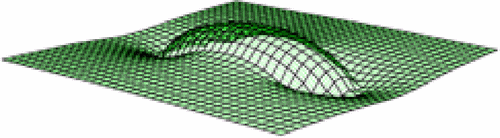
\includegraphics[scale = 0.5]{figures/literature_review/interfacial_curvature.png}
    \caption{Quadropolar capillary interactions around prolate ellipsoidal particles caused by interfacial deformations 
             around the particle. \cite{loudet_capillary_2005} Reprinted Figure 4 with permission from
             Loudet et al, Phys. Rev. Letter., 94, 08301, 2003 Copyright 2025 by the American Physical Society.}
    \label{fig:anisotropic_particle_interface}
\end{figure}


Anisotropic particles exhibit shape-dependent interfacial behavior due to their ability to deform fluid interfaces while maintaining zero mean curvature, satisfying the Young-Laplace equation 
(Figure~\ref{fig:anisotropic_particle_interface}) \cite{loudet_capillary_2005, cheng_shape-anisotropic_2013}. These deformations generate multipolar capillary interactions, which can be harnessed 
for curvature-guided migration and directed assembly at fluid interfaces \cite{cavallaro_curvature-driven_2011, read_dimerization_2020, sharifi-mood_curvature_2015}. Simulations have shown that 
ellipsoidal particles can adopt multiple metastable orientations depending on external perturbations and interfacial constraints \cite{gunther_lattice_2013}. When used as stabilizers in bijels, 
ellipsoidal particles produce finer domains than spherical particles at equivalent volume fractions, a result of their higher surface area-to-volume ratio and more efficient interfacial coverage 
\cite{gunther_timescales_2014}.

The dynamics of ellipsoid-stabilized bijels are distinct from their spherical counterparts, displaying two characteristic timescales. Initially, particles adsorb and align with the interface, 
followed by a slower reorganization phase driven by capillary interactions between particles \cite{gunther_timescales_2014}. Experimental results confirm that the domain size in rod- and ellipsoid-stabilized 
bijels still follows the scaling law $L \propto \frac{1}{\phi_p}$, though the proportionality constant depends on particle geometry \cite{hijnen_bijels_2015, madivala_exploiting_2009, daware_emulsions_2015}.

The geometry of the stabilizing particles plays a key role in determining rheological behavior. Madivala et al. showed that Pickering emulsions stabilized with rod-like particles had enhanced stability under 
shear, with greater resistance observed as particle aspect ratio increased \cite{madivala_exploiting_2009}. This enhancement was attributed to improved interfacial coverage and capillary interactions induced by 
interface deformations, which reinforced the particle monolayer. Similarly, emulsions stabilized by graphene nanosheets exhibited higher viscosity and viscoelasticity compared to those stabilized by spherical 
particles, underscoring the importance of particle shape \cite{imperiali_simple_2014}. The elasticity of the interface has also been shown to depend on the nature of the particle stabilizer used 
\cite{sun_assembly_2013}.

The rheological properties of bijels are of fundamental importance due to their direct influence on both fabrication and application. For instance, STrIPS fabrication relies on the controlled flow of a 
casting mixture into a solvent bath, necessitating precise knowledge of the material's rheology to optimize processing parameters \cite{haase_situ_2016, haase_continuous_2015}. In applied systems such as 
cross-flow reactors, the mechanical stability of the particle monolayer is critical; failure under shear or compositional gradients can limit performance \cite{boakye-ansah_controlling_2020}. Under constant 
shear, bijels exhibit shear-thinning behavior, which at moderate shear rates is well described by the Herschel-Bulkley model \cite{macmillan_rheological_2019, wang_morphology_2023}. At higher shear rates, the 
internal structure of the bijel is disrupted, leading to a transition toward Newtonian flow behavior \cite{cai_bijels_2017, bonaccorso_shear_2020}.

\begin{figure}
    \centering
    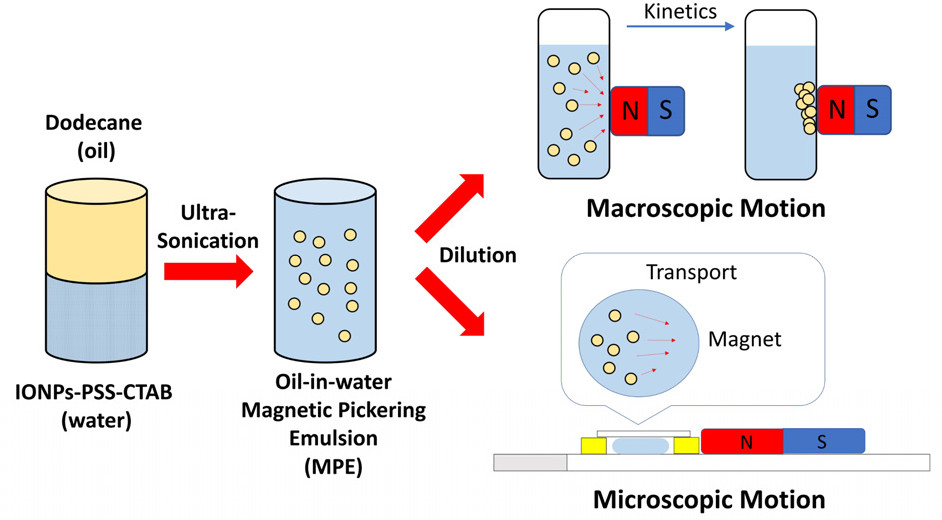
\includegraphics[scale = 1.5]{figures/introduction/magnetophoresis_emulsion.jpeg}
    \caption{Enhanced oil recovery of oil from water using magnetically responsive emulsion stabilizers, allowing for 
             locomotion and controlled coalescence of cargo from a matrix phase using magnetic fields. \cite{tham_magnetophoresis_2021} 
             K. Tham, W. M. Ng, S. S. Leong, S. P. Yeap, S. C. Low, H. L. Lee and J. Lim. Magnetophoresis of magnetic pickering 
             emulsions under low field gradient: Macroscopic and microscopic motion. 37, 1811: Reprinted (adapted) with permission from 
             Langmuir 2021, 37, 5, 1811-1822. Copyright 2025 American Chemical Society.}
    \label{fig:magnetophoresis_droplet}
\end{figure}

Introducing magnetic responsiveness into anisotropic particles offers a non-invasive strategy for controlling their behavior at fluid interfaces. Such particles can be fabricated via surface deposition of 
magnetic materials or synthesized as core-shell structures with magnetic cores and non-magnetic shells \cite{fei_magneto-capillary_2020, nakayama_stimuli-responsive_2018}. The interplay between magnetic 
torque and capillary anchoring governs particle orientation in response to external magnetic fields. According to Bresme-Faraudo theory, a neutrally wetting ellipsoidal particle at an interface experiences 
competing forces: the magnetic field seeks to reorient the particl's magnetic dipole moment, while capillary forces resist deformation away from the interface plane 
\cite{bresme_orientational_2007, davies_interface_2014}.

\begin{figure}
    \centering
    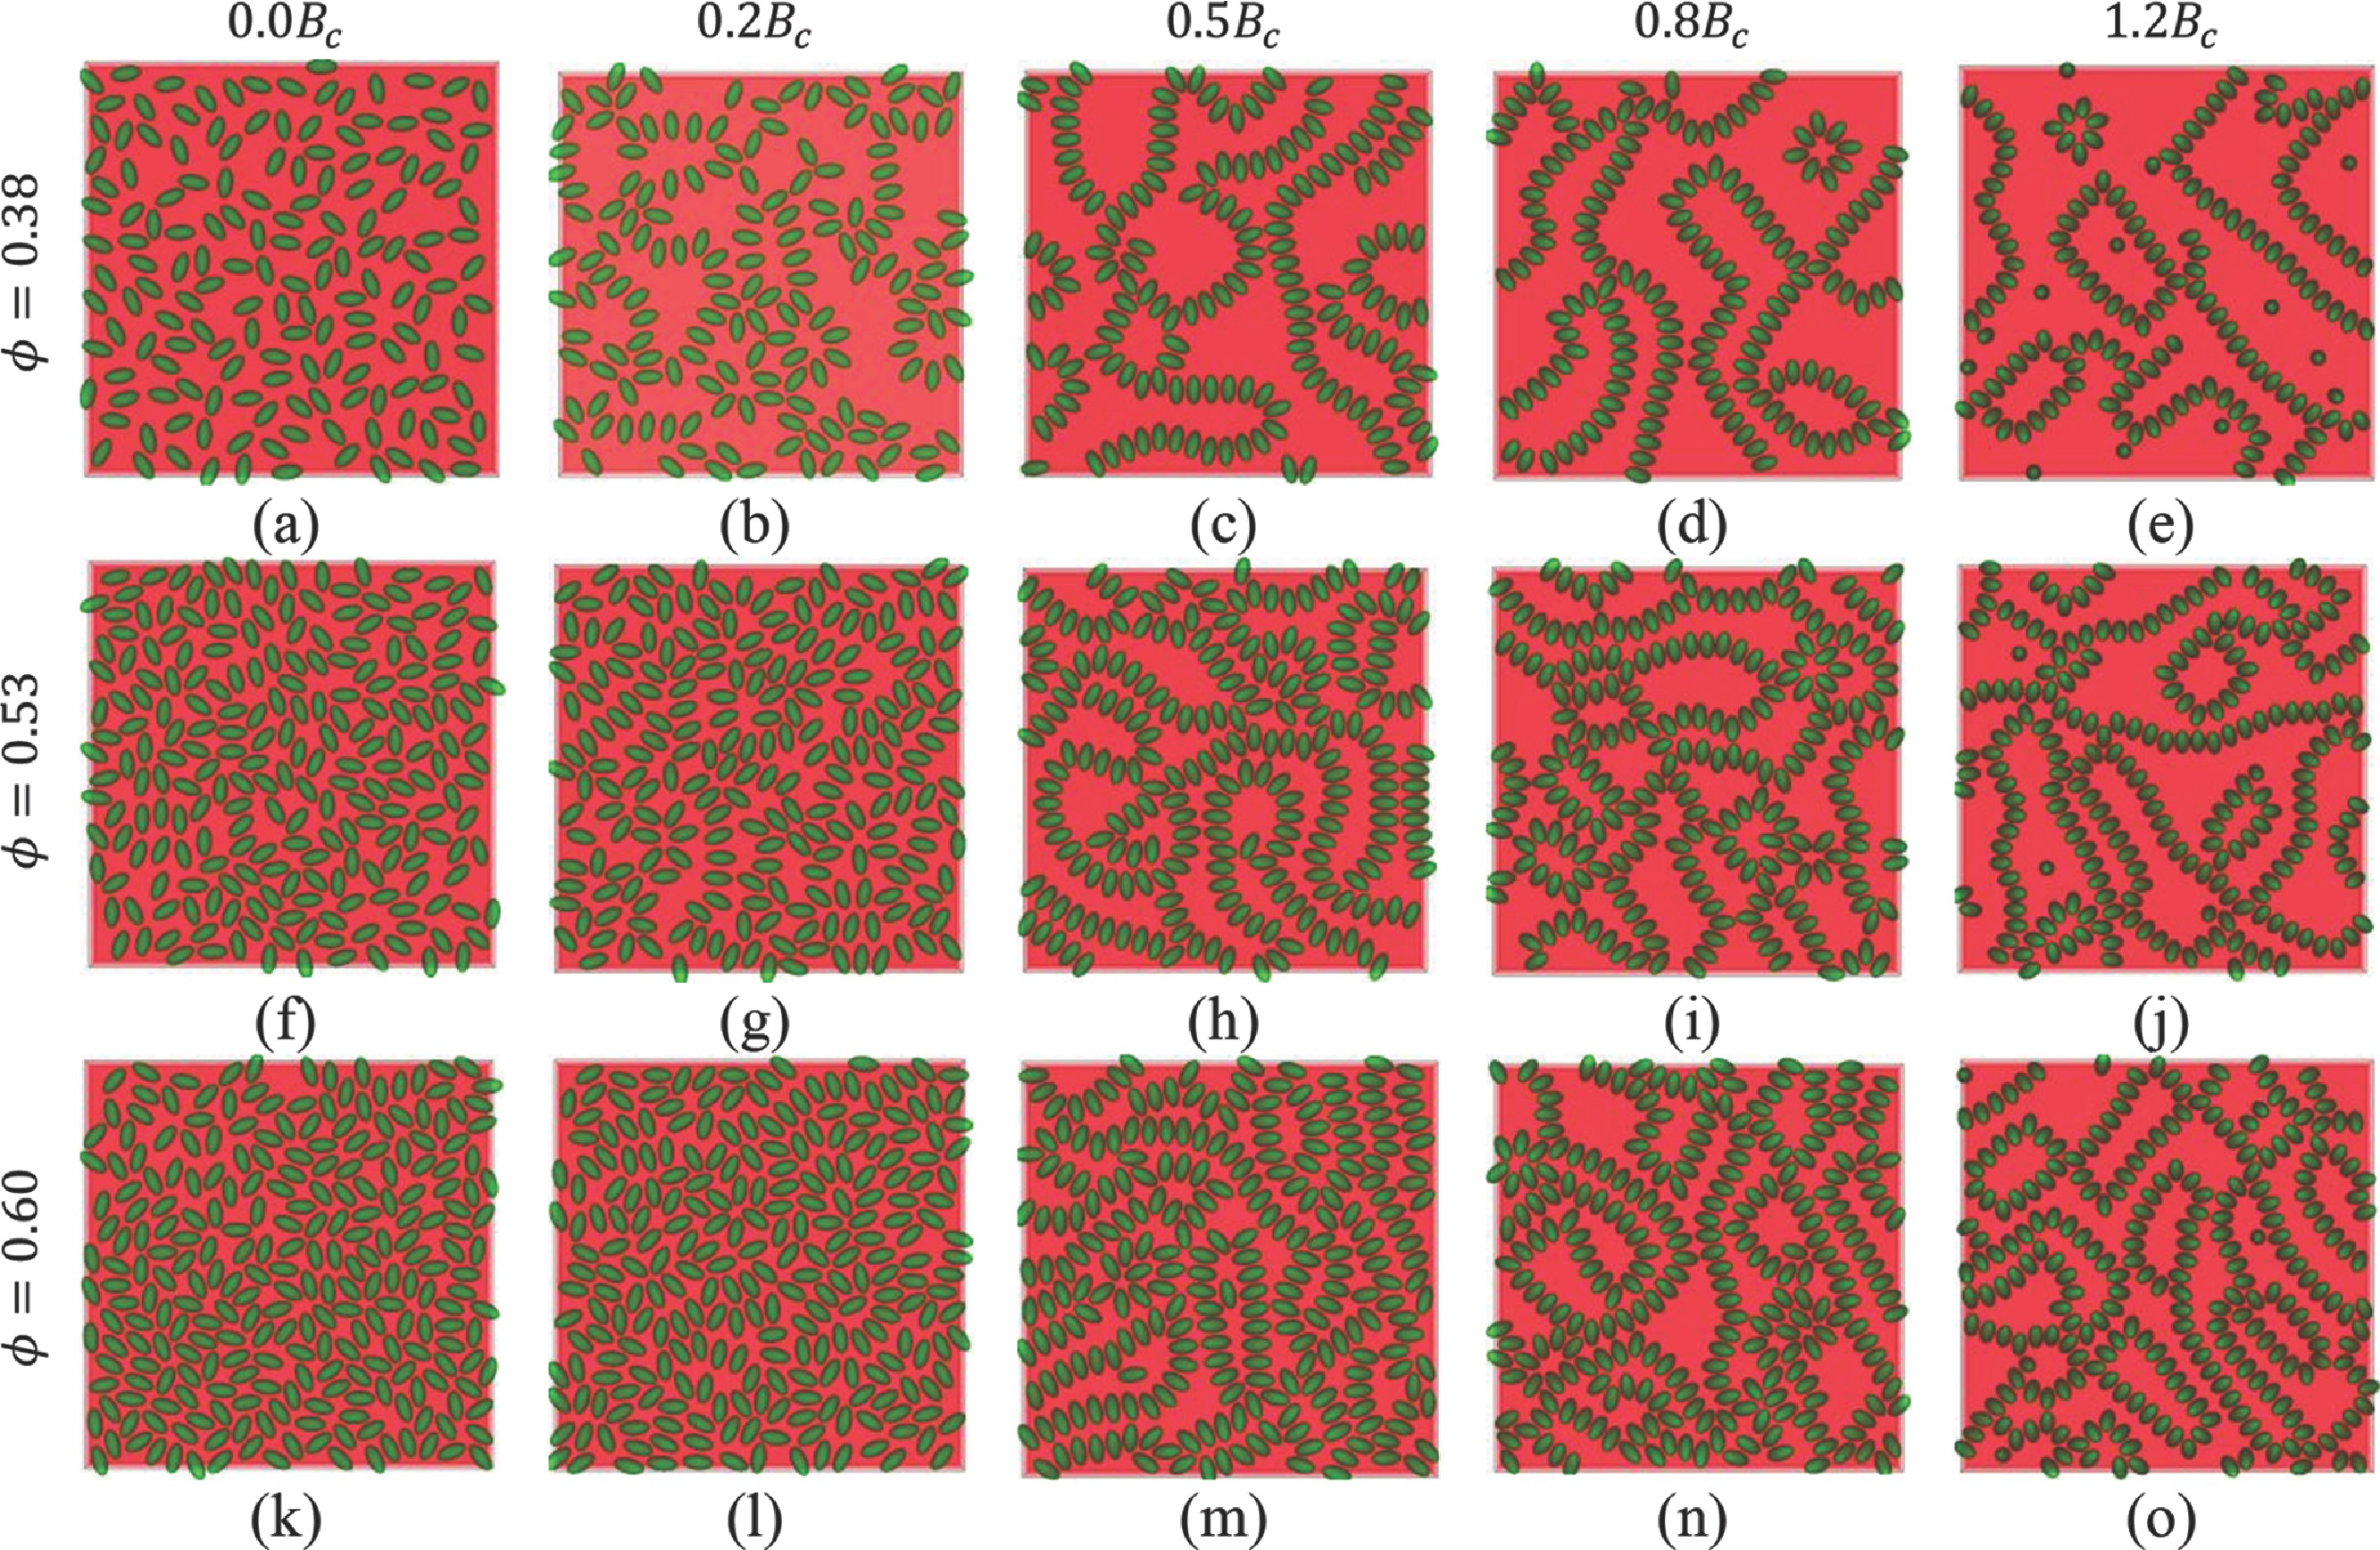
\includegraphics[scale = 0.4]{figures/introduction/anisotropic_particles_assembly.jpg}
    \caption{Assembly of prolate particles on a flat interface at various interfacial coverages and field strengths,
             showing the self assembly into chains that ellipsoidal particles can undergo under applied magnetic fields at
             interfaces. \cite{davies_assembling_2014} Reproduced from Davies et al. Adv. Mater., 26: 6715-6719 under the 
             Creative Commons CC BY license.}
    \label{fig:anisotropic_assembly}
\end{figure}

The equilibrium and metastable orientations adopted by anisotropic particles are functions of particle aspect ratio, surface wettability, and interfacial tension 
\cite{morgan_understanding_2013, newton_influence_2014}. Studies on superellipsoidal hematite particles at oil-water interfaces demonstrate multiple stable and metastable states, where particles align 
their major or minor axes relative to the interface depending on their geometry and energy landscape. Lattice Boltzmann simulations support these observations, showing how shape influences immersion 
depth and contact angle, which in turn affect orientation stability. Magnetic fields can perturb these equilibria by exerting torque on the particles, reorienting them along the field direction. 
Experiments confirm that magnetic ellipsoids can be reconfigured at the interface, enabling controlled switching between metastable and stable configurations.
As more particles interact under a magnetic field, their mutual dipolar interactions lead to the formation of linear chains or clusters on flat interfaces \cite{davies_assembling_2014, newton_capillary_2018}. 
The final arrangement is influenced by particle concentration, field strength, and local capillary geometry. In Pickering emulsions, these effects enable magnetically triggered droplet deformation, coalescence, 
and motility, demonstrating the potential for real-time, field-controlled manipulation of interfacial structures \cite{melle_pickering_2005, tham_magnetophoresis_2021}.

Magnetically responsive Pickering emulsions offer an additional layer of tunability. When a magnetic field is applied, particles reorient and organize at the interface, significantly altering the material's 
rheological response \cite{qiao_magnetorheological_2012, melle_pickering_2005}. This field-induced ordering can lead to reversible transitions between fluid-like and gel-like states, enabling on-demand control 
over flow properties. Such behavior is particularly advantageous for applications in enhanced oil recovery, drug delivery, and soft robotics, where adaptable and reconfigurable materials are essential 
\cite{tham_magnetophoresis_2021}.

This dissertation investigates the potential of magnetically responsive ellipsoidal particles to enable stimuli-responsive control over bijel microstructure. Specifically, it examines whether magnetic fields 
applied during or after bijel formation can induce meaningful structural changes, and how these changes, in turn, influence the rheological behavior of the resulting material. The central hypothesis is that 
particle reorientation under magnetic fields alters interfacial packing, ultimately reshaping domain morphology. 
Moreover, Carmack and Millet identified that the formation of particle chains was shown to play a critical role in phase separation dynamics. These chains acted as nucleation sites, guiding the development of 
fluid domains and influencing average channel diameter and particle localization at interfaces. These findings suggest that external fields, particularly when coupled with anisotropic particles, offer a 
promising route toward responsive and reconfigurable bijel architectures.
The remainder of this dissertation is organized as follows. Chapter 2 details the physics being modeled and the simulation methods used to model these physics, including the Lattice Boltzmann approach 
and magnetic dipole modeling. Chapter 3 investigates the effects of magnetic fields applied during bijel formation, analyzing their influence on domain structure and particle orientation. 
Chapter 4 investigates the microstructure of bijels stabilized by ellipsoidal particles under magnetic fields in more detail, providing further detail on the influence of the magnetic field on
the coarsening dynamics of the bijel.
Chapter 5 explores 
post-formation responsiveness, specifically examining particle unjamming and reordering phenomena. Chapter 6 assesses the rheological implications of these structural changes, with particular attention to 
yield stress and shear-thinning behavior. Finally, Chapter 7 summarizes the key findings, discusses their implications for the design of tunable porous materials, and outlines potential directions for future 
research.

% To explore this possibility, Kim et al. employed a free-energy-based Lattice Boltzmann method coupled with particles and external magnetic fields to study the responsiveness of bijels stabilized by 
% spherical particles \cite{kim_bijels_2010}. Their simulations showed that even under strong magnetic fields, the particles aligned with the field direction but did not meaningfully disrupt the 
% interfacial morphology. This result suggests that the isotropic geometry of spherical particles does not impart anisotropic stresses on the interface, thereby preserving the original structure of 
% the bijel despite external perturbations.


% Further computational work by Jansen and Harting expanded upon these findings by investigating the effects of fluid composition, surface tension, particle volume fraction, and particle contact angle 
% using a Lattice Boltzmann framework \cite{jansen_bijels_2011}. They found that while surface tension and fluid density had only minor effects on the resulting microstructure, the particle 
% volume fraction had a significant impact, with the characteristic length scale of the bijel inversely proportional to the particle concentration ($L \propto \frac{1}{\phi_p}$). Additionally, they 
% demonstrated that the formation of a bijel versus a conventional Pickering emulsion was primarily determined by the contact angle of the stabilizing particles and the relative fluid volumes, rather 
% than particle concentration alone. 

% However, as will be shown in the remainder of this review, modern fabrication approaches have increasingly 
% shifted away from TIPS in favor of alternative strategies.


% Further investigations into bijel microstructure have employed topological, geometric, and image analysis techniques to quantitatively characterize their complex morphology. Topological methods
% focus on properties such as genus and channel size distribution, which reveal differences in interfacial connectivity and structural complexity \cite{chan_channel_2012}. For instance, Chan and 
% Thornton compared bicontinuous structures generated using the Cahn-Hilliard and Allen-Cahn equations, highlighting key topological distinctions between these phase-separation models. The main strength 
% of topological approaches lies in their ability to assess both the shape and the interconnectedness of the structure.

% Geometric techniques, such as curvature analysis, offer insights into how factors like particle size and quench rate influence bijel formation. Reeves et al. used Gaussian curvature measurements to 
% compare bijels stabilized with micro- versus nanoparticles, demonstrating that smaller particles promote more negative Gaussian curvature and better approximation of minimal surface structures 
% \cite{reeves_particle-size_2015,reeves_quantitative_2016}. This finding is consistent with the notion that bijel interfaces resemble minimal surfaces, which are characterized by zero mean curvature 
% and negative Gaussian curvature \cite{jinnai_interfacial_2001}. Because nanoparticles more readily conform to curved interfaces without significantly disrupting interfacial geometry, they enhance 
% stabilization in regions with saddle-like curvature \cite{reeves_quantitative_2016}.

% Image analysis techniques have also been instrumental in characterizing features such as pore size distribution, tortuosity, connectivity, and self-similarity of bijel networks 
% \cite{mcdevitt_microstructural_2019,reeves_quantitative_2016}. These methods utilize tools like region-growing and labeling algorithms (e.g., Hoshen-Kopelmann), segmentation techniques, and watershed 
% transforms to extract quantitative metrics from imaging data. For example, pore size distributions can be derived from watershed algorithms, while connectivity is assessed using segmentation-based 
% approaches.



% Recent advances suggest that anisotropic particles, particularly ellipsoidal particles, may offer enhanced responsiveness due to their shape-dependent 
% interfacial behavior. When subjected to magnetic fields, ellipsoidal particles can align directionally, inducing local anisotropy in the interfacial 
% packing arising from capillary deformation of the interface. This property has been characterized to induce self assembly of particles, 
% shown in Figure \ref{fig:anisotropic_particle_interface} 
% \cite{bresme_orientational_2007, davies_assembling_2014, newton_influence_2014}. By utilizing the magnetic field driven re-orientation and self assembly 
% of particles at interfaces, the microstructure of bijels could be influenced pre and post formation. Therefore, leveraging this behavior offers a 
% pathway to decouple microstructure control from casting mixture composition, expanding the design space for bijel derived porous materials and
% soft matter.

% Stimuli-responsive strategies offer an attractive alternative for post-synthetic or in-situ control of bijel microstructures. External fields, 
% pH, and temperature have all been explored to modify emulsion morphologies, particularly in Pickering emulsions 
% \cite{tham_magnetophoresis_2021, cui_stabilizing_2013}. In Pickering emulsions, magnetically responsive particles have enabled droplet
% manipulation, deformation, and coalescence control, shown in Figure \ref{fig:magnetophoresis_droplet}. By contrast, similar stimuli-responsive 
% behaviors in bijels remain underexplored. Prior work with spherical particles under magnetic fields has shown limited microstructural modification 
% \cite{kim_bijels_2010}, while electric fields have demonstrated greater influence \cite{carmack_tuning_2018}.

% Over the past decade, advancements in synthesis techniques have significantly expanded the ability to fabricate particles with anisotropic geometry and surface chemistry. 
% The choice of synthesis method depends on the desired particle shape. For example, ellipsoidal particles can be readily produced through the mechanical deformation of 
% % NOTE: This paragraph introduces a new concept—consider explicitly linking it to the prior paragraph (e.g., 'Beyond traditional surfactants...').
% polymer spheres, while dumbbell-shaped particles can be synthesized using microfluidic devices or emulsion templating. \cite{fei_magneto-capillary_2020} 
% Square-shaped particles, on the other hand, can be 
% generated through controlled crystallization \cite{morgan_understanding_2013}. The increasing variety of synthesis methods has reduced geometric constraints when exploring 
% potential particle stabilizers for bijels \cite{wu_recent_2016}.



% Magnetic fields offer a non-invasive and targeted method for manipulating the behavior of particles. Magnetic particles can be fabricated from
% coatings applied onto particles through deposition techniques or a core-shell particle that encapsulates a magnetic core with a non-magnetic shell. 
% \cite{fei_magneto-capillary_2020, nakayama_stimuli-responsive_2018} These effects arise due to the interplay between the magnetic torque or force 
% acting on the particles and the capillary interactions that govern their behavior at the interface. One theory developed for neutrally wetting ellipsoidal 
% particles is Bresme-Faraudo theory. \cite{bresme_orientational_2007, davies_interface_2014}
% A wide range of behaviors has been observed when magnetic fields are applied to interfacial particles. Individual particles tend to align their magnetic 
% dipole moments along the direction of the field, causing them to reorient relative to the interface. \cite{kim_bijels_2010}
% For anisotropic particles such as ellipsoids, this results in a tilt or rotation that changes their interfacial footprint and local curvature. 
% \cite{davies_assembling_2014, davies_interface_2014} The orientation of the particle is a function of the capillary interactions with the interface that 
% prefers to keep the particle flat on the interface and the magnetic field that is attempting to rotate the particle out of the interface. The magnetic force
% experienced by the particle is a function of the applied field strength, magnetic susceptibility, size of the particle, shape of the particles 
% and aspect ratio of the particle. 



% The rheological properties of bijels are of fundamental importance due to their direct influence on both fabrication and application. For instance, STrIPS fabrication relies on the controlled 
% flow of a casting mixture into a solvent bath, necessitating precise knowledge of the material's rheology to optimize processing parameters \cite{haase_situ_2016, haase_continuous_2015}. In 
% applied systems such as cross-flow reactors, the mechanical stability of the particle monolayer is critical; failure under shear or compositional gradients can limit performance 
% \cite{boakye-ansah_controlling_2020}.

% Under constant shear, bijels exhibit shear-thinning behavior, which at moderate shear rates is well described by the Herschel–Bulkley model \cite{macmillan_rheological_2019, wang_morphology_2023}. 
% At higher shear rates, the internal structure of the bijel is disrupted, leading to a transition toward Newtonian flow behavior \cite{cai_bijels_2017, bonaccorso_shear_2020}. 
% Figure~\ref{fig:bijel_under_shear} illustrates this phenomenon, showing that under shear, particles initially align with the flow direction before detaching from the interface 
% \cite{bonaccorso_shear_2020}. This behavior is consistent with findings in colloidal suspensions, where hard-sphere systems undergoing shear exhibit shear banding and particle ordering along 
% the flow direction, resulting in pronounced shear thinning \cite{vermant_flow-induced_2005, brader_nonlinear_2010}.

% Bijels have also been shown to exhibit gel-like behavior, particularly when the storage modulus exceeds the loss modulus, indicating a dominant elastic response \cite{lee_making_2013, bai_dynamics_2015}. 
% Ching and Mohraz proposed that bijels behave similarly to 2D colloidal glasses percolating in 3D space, based on comparisons of their linear viscoelastic responses to those of attractive colloidal gels 
% \cite{ching_bijel_2022}. Hallmarks of colloidal glass behavior include the presence of a yield stress (the point at which irreversible deformation occurs), viscoelasticity (a combination of solid- and 
% liquid-like behavior), and a dramatic slowdown in dynamics at the glass transition point \cite{pham_yielding_2008, weeks_introduction_2017}.

% The geometry of the stabilizing particles plays a key role in determining rheological behavior. Madivala et al. showed that Pickering emulsions stabilized with rod-like particles had enhanced stability 
% under shear, with greater resistance observed as particle aspect ratio increased \cite{madivala_exploiting_2009}. This enhancement was attributed to improved interfacial coverage and capillary interactions 
% induced by interface deformations, which reinforced the particle monolayer. Similarly, emulsions stabilized by graphene nanosheets exhibited higher viscosity and viscoelasticity compared to those stabilized 
% by spherical particles, underscoring the importance of particle shape \cite{imperiali_simple_2014}. The elasticity of the interface has also been shown to depend on the nature of the particle stabilizer 
% used \cite{sun_assembly_2013}.

% Magnetically responsive Pickering emulsions offer an additional layer of tunability. When a magnetic field is applied, particles reorient and organize at the interface, significantly altering the material's 
% rheological response \cite{qiao_magnetorheological_2012, melle_pickering_2005}. This field-induced ordering can lead to reversible transitions between fluid-like and gel-like states, enabling on-demand 
% control over flow properties. Such behavior is particularly advantageous for applications in enhanced oil recovery, drug delivery, and soft robotics, where adaptable and reconfigurable materials are 
% essential \cite{tham_magnetophoresis_2021}.


% While not strictly stimuli-responsive, microstructure modifications have been achieved by applying a particle volume fraction gradient during the formation of 
% bijels using Thermally Induced Phase Separation (TIPS). \cite{french_bicontinuous_2022} In their study, French et al. allowed particles to partially sediment in the bijel casting mixture
% before initiating thermal quenching. The gradient in particle volume fraction along the height of the reaction vessel caused the jamming point of the bijel
% to vary along the gradient axis, causing a channel size gradients of up to 2.8\% per millimeter, as measured using confocal microscopy.